\documentclass[conference]{IEEEtran}
\IEEEoverridecommandlockouts
% The preceding line is only needed to identify funding in the first footnote. If that is unneeded, please comment it out.
\usepackage[UTF8, heading = false, scheme = plain]{ctex}
\usepackage{cite}
\usepackage{amsmath,amssymb,amsfonts}

\usepackage{graphicx}
\usepackage{textcomp}
\usepackage{xcolor}
\usepackage{algorithm} 
%\usepackage{algorithmic}
\usepackage{algpseudocode}

\renewcommand{\algorithmicrequire}{ \textbf{Input:}}
\renewcommand{\algorithmicensure}{ \textbf{Output:}} 
\def\BibTeX{{\rm B\kern-.05em{\sc i\kern-.025em b}\kern-.08em
    T\kern-.1667em\lower.7ex\hbox{E}\kern-.125emX}}
\begin{document}
\title{Incremental Mutual Feedback Learning to Chinese Segmentation and Named Entity Recognition in Electronic Medical Record\\
%{\footnotesize \textsuperscript{*}}
\thanks{*Kenny Q. Zhu is the contact author and is partially supported by NSFC grants  91646205.}
}

\author{
\IEEEauthorblockN{1\textsuperscript{st} }
\IEEEauthorblockA{\textit{Department of Medical Artificial Intelligence} \\
\textit{Synyi AI}\\
Shanghai, China \\
@synyi.com}
\and
\IEEEauthorblockN{2\textsuperscript{nd} }
\IEEEauthorblockA{\textit{Department of Medical Artificial Intelligence} \\
\textit{Synyi AI}\\
Shanghai, China \\
@synyi.com}
\and
\IEEEauthorblockN{3\textsuperscript{rd} }
\IEEEauthorblockA{\textit{Department of Computer Science and Engineering} \\
\textit{Synyi AI}\\
Shanghai, China \\
@synyi.com}
\and
\IEEEauthorblockN{4\textsuperscript{th} }
\IEEEauthorblockA{\textit{Department of Computer Science and Engineering} \\
\textit{Shanghai Jiao Tong University}\\
Shanghai, China \\
@synyi.com}
}

\maketitle

\begin{abstract}
We present an incremental mutual feedback framework to perform Chinese Word Segmentation (CWS)  and Name Entity Recognition (NER) using incremental learning with efficient decoding method. We implement a novel Long Short Term Memory (LSTM) Networks model  BiLSTM-CRF for both tasks. Based on the idea of BiLSTM-CRF model, a variant Beam Search decoder is adopted to the dynamic feedback framework as opposed to traditional tagging approach. In addition, by obtaining error information from NER task, we developed an error-driven learning approach to capture the interdependency among segmentation and name entity recognition to further improve the system. Experiments on electronic medical records corpora demonstrate that our work efficient and effective compared with the strong pipelined baseline and best-reported joint learning model.The framework  F-score achieved 2.46\%improvement for segmentation and 0.24\% improvement for recognition, compared with each of the two tasks alone.
\end{abstract}

\begin{IEEEkeywords}
Medical Concepts, Mutual Feedback Learning, BiLSTM-CRF, Variant Beam Search
\end{IEEEkeywords}

\section{Introduction}
Electronic medical records are widely used in healthcare research for exploratory and predictive analytics\cite{b1}. While various methods have been developed for English medical records, rare models have been establish for Chinese medical records\cite{b2,b3,b4,b5}.  On the other hand, the large amount of information contained in Chinese medical texts will benefit the field of biomedical informatics. The success of extracting knowledge from medical notes often requires the application of natural language processing (NLP) techniques. Word segmentation\cite{b6,b7} and named entity recognition\cite{b8,b9} are considered as two fundamental issues for Chinese medical text processing. Different from most European languages, there is no space separating two different words. Therefore, Chinese word segmentation is the first step for Chinese language processor. For instance, the sentence ‘两肺弥漫性病变 ,考虑急性间质性炎症可能(Two lung diffuse lesions, considering the possibility of acute interstitial inflammation)’ should be segmented as ‘两肺 (two lung)/弥漫性病变(diffuse lesions)/,(,)/考虑( considering)/急性间质性炎症 (acute interstitial inflammation)/可能(possibility)’ . The second step involves named entity recognition from medical text. In our work, we consider the following three categories of named entities: (1) disease like ‘肺炎(pneumonia)’; (2) medical tests and assays like ‘血压(blood pressure)’ ; and (3) treatments like ‘化疗(chemotherapy)’. In the example sentence above, the phrase ‘急性间质性炎症 (acute interstitial inflammation)' should be extracted as an entity of type ‘disease’. 

The traditional pipeline approach treat word segmentation and named entity recognition as separated two tasks\cite{b10,b11,b12}. However, there's a significant relation between two task. Given a NER term like ‘慢性肾小球肾炎(chronic glomerulonephritis)',  CWS tool can separate it into three words as ‘慢性(chronic)/肾小球(glomerulus)/肾炎(nephritis)' . The component of the NER  should have a certain semantic meaning and not be allowed to contain a fraction of a word. The result of CWS task can influent the performance of subsequent NER task. The  pipeline approach creates word segmentation first and then feeds the segmented words into NER task. It is straightforward, but CWS tools built on open source annotated corpus works badly on medical text. It suffers from error propagation since an incorrect word segmentation would cause an error in the NER stage. The joint-learning approach \cite{b6, b13,b14} overcomes this drawback. It trains a model to learn both word segmentation and the NER task at the same time. However, the joint-learning process generally assumes the availability of manual word segmentations for the training data, which limits the use of this approach. Joint-learning also share large mount of parameters, which makes the train process slow. Annotated domain data is scarce due to high cost.

In this paper, we develop a novel  a mutual feedback learning approach which can feedback the error information from NER stage to modify the segmentation result dynamically. BiLSTM-layer is trained first for CWS, then CRF layer with variant Beam Search decoder will be used to decode the tags. During the training processing, we judge the NER label to find error segmentation area and feedback them to decoder. We also adopt a mapping concept knowledge base to find the potential error mention boundary and develop a segment-based decoding algorithm on BiLSTM-CRF framework. Assignments for the same sentence with wrong mention boundary information in the next stage is considered simultaneously during search.

The main contributions in this paper are as follows. First, this is the first work to incrementally predict word segmentation and entity mentions using a BiLSTM-CRF mutual feedback framework. Second, we furthermore proposed a new variation of beam search to avoid wrong path on segment-level. Third, we create a mapping concept knowledge base to capture wrong mention boundaries.  Finally, to the best of our knowledge, our work is the first to dynamically learn error information from next step to improve two individual task in medical records.

Experimental results show that the proposed framework achieves better performance than pipelined baseline and joint approach, and map concept database provide further significant gains.

\section{Methods}
\subsection{The Mutual Feedback Framework}
The framework of our work is shown in Fig.~\ref{fig:framework}. We input a set of sentences with Chinese characters and  tags as training data. Then, LSTM \cite{b15,b16} will train the embeddings and use these vectors to get the final model in CRF layer. The segmentation of sentences to be labeled with NER  will be fed as features when training the model. Then we use BiLSTM-CRF \cite{b17} to get the NER result of input sentences. If the NER result can not be found in map concept part, we the result is wrong and return the wrong places to the segmentation part. The segmentation part will catch the information of wrong part and decode the sentences again to find the best result. 
\begin{figure}[htbp]
\centerline{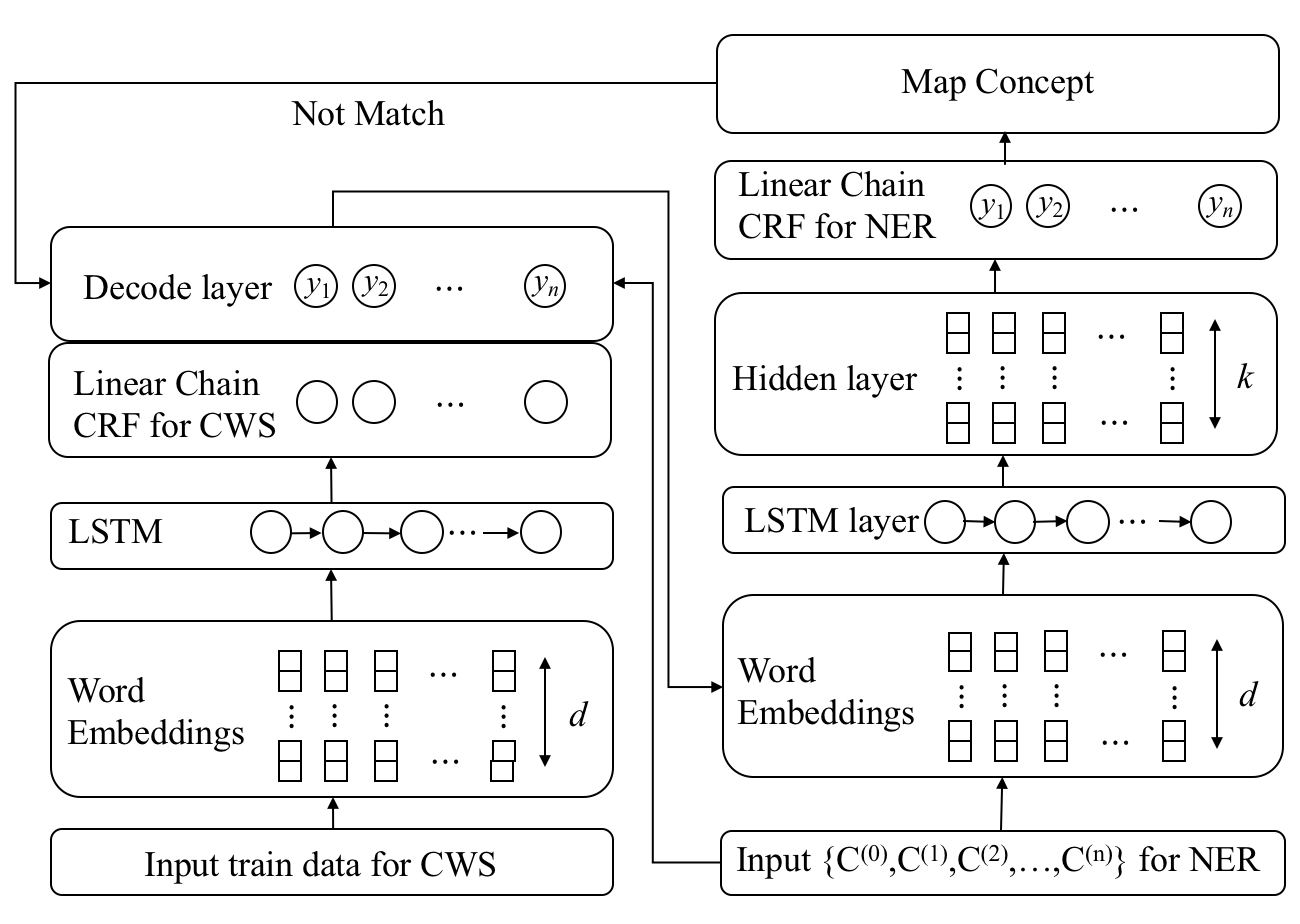
\includegraphics[height=6cm ,width=9cm]{framework.png}}
\caption{Mutual Feedback Framework.}
\label{fig:framework}
\end{figure}

\subsection{BiLSTM-layer Chinese Word Segmentation}
The recurrent neural network(RNN) has become increasingly popular due to the improvement of GPU and various different neural network algorithms proposed.  A  a single layer, left to right LSTM for Chinese word segmentation is a recurrent neural network (RNN) which uses a series of gates(input gate$(i)$, forget gate$(f)$ and output gate$(o)$) and  memory cell$(c)$ to control how memory is propagated in the hidden states of the model. For each time step $t$ and a given input $x_t$, we update hidden layer by using equation $(1)$ to $(5)$.
\begin{equation}
i_t=\sigma(W_i \cdot[h_{t-1},x_t] + b_i )\label{eq}
\end{equation}
\begin{equation}
\widetilde{C_t}=tanh(W_c\cdot[h_{t-1},x_t] +b_C)\label{eq}
\end{equation}
\begin{equation}
C_t=f_t\ast C_{t-1}+i_t\ast \widetilde{C_t}\label{eq}
\end{equation}
\begin{equation}
o_t=\sigma(W_o \cdot[h_{t-1},x_t] + b_o )\label{eq}
\end{equation}
\begin{equation}
h_t=o_t\ast tanh(C_t)\label{eq}
\end{equation}

Chinese word segmentation is often treated as a sequence tagging task on character level. Each Chinese character is initialized as a d dimensional vector, which the LSTM will modify during its training time. These vectors are then use BIES tagging scheme to represent \textbf{B}egin, \textbf{I}nside, \textbf{E}nd, and \textbf{S}ingleton. For a given input sentence with n characters 
$$X = \{x_1,x_2,..., x_n\}$$

Each word $x_i$ in a sentence can be computed a representation $forward\_h_{x_i}$ that the former text expression by LSTM. In addition to considering past information from left, Bidirectional LSTM also captures future information from the right of the token.

\subsection{CRF-layer}
When there is a correlation between the labels, we can use condition random field (CRF) to learn the global information effectively.  For a sequence $x$ containing $n$ words that the $p^{th} $ word is entered into bidirectional LSTM to acquire a feature representation $h_p$, so we can get a flowing sequence $h=(h_1,h_2,...,h_p,...,h_n)$ . Then we define a score matrix $P$, which is an output result of bidirectional LSTM. $P$ is of size $n\times k$, where $k$ the number of is different labels, and $P_{i,j}$ denotes the score of the $j^{th}$ label of the $i^{th}$ word.

For a sequence of predicted labels $y = (y_1,y_2,...,y_n)$, we use (6) to define its score.

\begin{equation}
f(h,y)=\sum_{i=0}^{n}M_{y_i,y_{i+1}}+\sum_{i=1}^{n}P_{i,y_i}\label{eq}
\end{equation}

Where M is a matrix of transition scores such that $M_{i,j}$ represents the score of a transition from the label to label. The first part of the equation represents the transfer feature, and the latter part represents the state feature. We add start and end tag to the set of possible tags and they are the tags of $y_0$ and $y_n$ that separately means the start and the end symbol of a sentence. Therefore, $M$ is a square matrix of size $k + 2$. After applying a softmax layer over all possible tag sequences, the probability of the sequence $y$:
\begin{equation}
p(y|h) = \frac{e^{f(h,y)}}{\sum_{\widetilde{y} \in Y_h}e^{f(h,\widetilde{y})}}\label{eq}
\end{equation}

Whenever given a feature $h$ of the candidate instance and a label sequence $y$ that we can use (7) to maximize target function by the CRF label.

\begin{equation}
log(p(y|h)) = f(h,y)-log\sum_{\widetilde{y}\in Y_h}e^{f(h,\widetilde{y})}\label{eq}
\end{equation}
Where $Y_h$ represents a set of all probable label sequences. While decoding, we predict the output sequence that gets the maximum score given by:
\begin{equation}
y^* = \mathop{\arg\max}_{\widetilde{y} \in Y_h} f(h,\widetilde{y})\label{eq}
\end{equation}

\subsection{Decoding Algorithm}
One main challenge to search for Chinese word segmentation incrementally is catching the information of error from subsequent tasks. We employ the idea that each state corresponds to a segment of the input sequence. It presents a variant of Viterbi algorithm for exact inference in linear-CRF. We relax the wrong token boundary with before or after one word length and relax max operation by beam-search. As shown in {alg:A}, Let $\widehat{d}$ be the upper bound of word length. The k-best partial assignments ending at the $i-th$ Chinese character for wrong segment can be calculated as:

\begin{equation}
B[i]=\mathop{k\text{-}BEST}_{i \in index, y \in Y_h} log(p(y|h)) \label{eq}
\end{equation}

where $y_{[1:i−d]}$ stands for a partial configuration ending at the $(i-d)$-$th$ token, and $y_{[i−d+1,i]}$ corresponds to the structure of a segment with wrong position information (i.e., subsequence of $x$) $x_{[i−d+1,i]}$. For each token index $i$, it maintains a beam for the partial assignments whose last character end at the $i$-$th$ token. There are three kinds of actions during the search:

\begin{itemize} 
\item \textbf{Viterbi Decoding}
Here, we use path to represent labeling sequence. The aim of Viterbi algorithm is to find the sequence labeling path with maximum probability. For the sequence without wrong signal, we use Viterbi algorithm to get the sequence path. We initialize the probability of first character with potential labels in $Y_h$. Then we can get the score for each $h_i$ by calculating $log(p(y|h))$. The Viterbi algorithm gives the labeling path with maximum  score until meets the $h_i$ which is in the wrong labeling list.
  
\item \textbf{Variant Beam Search}
We set the beam size $k$. First, the algorithm enumerates all possible path for wrong segment  (i.e., subsequences) of x ending at the current character with various segmentation labels. Each path of wrong segment is then appended to existing partial assignments in one of the previous beams to form new assignments. Finally the top k results are recorded in the current beam.

\item  \textbf{Link} After the stage of regular Variant Beam Search, the algorithm looks backward to link previous wrong segment and remove the path with wrong information through NER stage. This processing is showing in Fig.~\ref{fig:Partially-labeled}. Red path represents the wrong path with the highest score. We pick up second highest path in top k path list.  After Regular Viterbi Decoding step, it only considers the previous highest path at previous one character. Then, enumerates all possible path as beam search stage.
\end{itemize}

In Viterbi Decoding, the observed sequence only need to be went through one time, so the complexity is $O(m)$. The time complexity for calculating score in each step is $O(4*4)$. So the total time complexity is $O(16m)$. The total time complexity for beam search is $O(16k*m)$.


\begin{algorithm}  
\caption{Variant Beam Search Decoder}  
\label{alg:A}  
\begin{algorithmic}[1] 

\Require 
\qquad 



$h = (h_1, h_2,..., h_i,..., h_m)$: 

input sentence representation 

$k$: beam size 

$E$: A matrix of unary potentials.

$Trans$: A matrix of binary potentials.

 

$S= (s_1,s_2,...,s_j,...,s_n) $: 

Record segmentation with wrong position
where 

$s_j=(seg_j, index_j)$
\Ensure 
\qquad 

$P$: Path of squence labels 

$V$: Viterbi Score 

\Function{Decoder}{$h,k,E,Trans,S$}
\State initialize $m$ empty beams $B[1..m][1..k]$
\State initialize the start state of squance $y_1$
\State initialize path $P[1..m]$
\State initialize the Viterbi score $V$
\For {$i \leftarrow 2...m$}
	\If  {$i$ and $i-1$ in $index$ of $S$}
		\State $B[i], V$=\Call{Beam}{$h$,$k$,$E$,$Trans$,$S$,$preP$,$V$}
	\ElsIf{$i$ and $i+1$ out of $index$}
		\State $P[i], V$=$Viterbi(h,E, Trans,preB,V)$
	\ElsIf  {$i$ in $index$ and $i-1$ out of $index$}
		\State $P[i], V$=$Link(h,k,E,Trans,S,preP,V,InB)$
	\ElsIf {$i$ in $index$  and $i-1$ out of  $index$}
		\State  $P, V$=$Link(h,k,E,Trans,S, preP,V,outB)$
	\EndIf
\EndFor
\State \Return $P, V$
\EndFunction

\Function{Beam}{$h$,$k$,$E$,$Trans$,$S$,$P$[$i$-1],$V$}
\State $P, V$ = $log(p(y|h))$ for each $h_i$
\State remove wrong path
\State sort all path by V
\State choose topk in B	
\State \Return $B[i],V$
\EndFunction

\Function {Viterbi}{$h,$E$, Trans,B[i$-$1],V$}
	  \State $P, V$ = $log(p(y|h))$ for each $h_i$
	  \State \Return $P, V$
\EndFunction

\Function  {Link}{$h,k,E,Trans,S, P[i$-$1],V,Case$}
	\State if (Case ==1)\{   
	\State calculating P, V = $log(p(y|h))$ for each $h_i$
	\State choose top k path with V
	\State return B[i], V
	\State elseif(case ==2) \{
	\State calculating P, V = $log(p(y|h))$ for each $h_i$
	\State choose top 1 path with V
	\State \Return P, V 
\EndFunction

\end{algorithmic}
\end{algorithm}

\begin{figure*}[htbp]
\centering
\centerline{\includegraphics[height=5.5cm ,width=15.5cm]{Partially-labeled.png}}
\caption{Partially-labeled word segmentations derived from error information in named entity labels..}
\label{fig:Partially-labeled}
\end{figure*}

\subsection{Error Driven Structured-Perceptron Learning}
Following the previous sections, we train our automatic word segmenter with BiLSTM-CRF model. This word segmenter achieves state-of-the-art or comparable performance. It uses word segmentation first and feeds the segmented words to subsequent NER task. We can keep using characters as the labeling units and also add the word segmentation information as additional features. Given the current character $c_0$ and word segmentation output represented as ‘$BIES$’  tag $t_0$, we extract the character features. The tag features provide word segmentation information indirectly to NER system.

To estimate the feature weights, we use Error Driven Structured-Perceptron (Collins, 2002), an extension of the standard perceptron for structured prediction, as the learning framework.Huang et al. (2012) proved the convergency of structured perceptron when inexact search is applied with violation-fixing update methods such as early update (Collins and Roark, 2004). Since we use variant beam-search in this work, we update $w$ when we do not map the right concept in $map\_concept$  database. In addition, we use averaged parameters to reduce overfitting as in (Collins, 2002).

\begin{algorithm}  
\caption{Adaptive Error-Driven Learning}  
\label{alg:A}  
\begin{algorithmic}[1] 
\Require
\qquad 

training set $D = \{(x^{(j)}, y^{(j)})\}^N_i=1$

maximum iteration number $T$

\Ensure
\qquad 

model parameters \textbf{w}

\State initialize $\textbf{w} \leftarrow 0$

\For {$t \leftarrow 1...T$}
	\For {$(x,y) \in D$}
		\State $(x, y', z) \leftarrow  Varient\_Beam\_Search(x,y,\textbf{w})$
		\If {$z \ne y$ or $map\_concept == 0$}
			\State $\textbf{w} \leftarrow \textbf{w} + f(x,y')-f(x,y)$
		\EndIf
	\EndFor
\EndFor
\State \Return \textbf{w}
\end{algorithmic}  
\end{algorithm} 


\subsection{Map Concept Rule}
In biomedical text, the entities are more complex and generally long such as some disease name '溃疡型低分化管状腺癌(Ulcerative low differentiated tubular adenocarcinoma)' composed of multiple words or multiple medical concepts. We develop a knowledge base which contains the component of different medical concepts. When getting the name entities result from our BiLSTM-CRF model, we will search the knowledge base to judge wether the concept of entities exits. If the concept not exits in knowledge base, we see it as an error entities. This information will be feedback to the segmentation part.

The knowledge base is a set of words with the same word concept meaning and the different short word with meaningful concept can comprise long word with new concept.
\section{Experiments}
\subsection{Data Preparation}
The three standard performance metrics, precision (P), recall (R) and F-measure (F), are used as evaluation metrics in our task.
In the experiment, we followed the standard leave-one-out method and the cross-validation method. In this paper, fivefold cross-validation and averaged metrics were used. 
We annotated medical datasets for our experiment and future research. The  dataset is electronic medical records (EMR) from our partner hospital. The data only permits noncommercial/academical use. The annotation was done by several doctors. It was carried out following a Chinese word segmentation criteria[7] created by Institute of Computational Linguistics at Peking University.  For Name Entity Recognition, the labelling standard is similar to the method in I2B2 Challenge 2010\cite{nn}
tasks. For quality control, annotators were trained until they achieve about 80\% inter-annotator agreement on previously annotated materials. Then we conducted double-blind annotation, with resolution of disagreements by a senior annotator. The entire annotation process follows \cite{nn}. We removed all names (of patients and hospitals), addresses, hospital numbers and EMR IDs in the original data to anonymize and de-identify it.

Also we do experiment on standard public data, we use the benchmark CWS and NER data from the third SIGHAN Chinese language processing Bakeoff (SIGHAN-3) \cite{nn}. It consists of 46,364 sentences in the training set and 4,365 sentences in the testing set. These data are annotated with both word segmentation label and NER information.
\subsection{Baseline System}
Two baseline methods are compared.

\textbf{Pipeline-BiLSTM-CRF} Both of the CWS and NER can be formulated as sequence labeling tasks, and can be solved using machine learning techniques such as Conditional Random Field (CRF), Recurrent Neural Network, or their combinations.
We adopt the tool BiLSTM-CRF segmenter and BiLSTM-CRF NER system as pipeline. In baseline system, each Chinese character is treated as a labeling unit.

\textbf{Joint-learning-BiLSTM-CRF} 
We proposed a joint model that was trained on combined labels.That is, instead of training two separate BiLSTM-CRF models for word segmentation and named entity recognition, we combined the sequential labels of the two tasks and trained a joint BiLSTM-CRF model that performs the two tasks simultaneously. Also, the word segmentation and NER training share all the parameters of the LSTM module.

\subsection{Results and Discussion}
We compare the mutual feedback framework with two baseline approach. The experimental results are shown in table 1. In general, mutual feedback framework achieved better results than pipeline method and joint
model on both tasks. The mutual feedback approach achieve an increase of 0.32\%, 5.91\% and 0.46\% on the
named entity recognition task for precision, recall and F1-Score.
Compared to the joint model using combined task labels,
the mutual feedback approach also achieved comparable performance on
the word segmentation task. Furthermore, as we have mentioned
in the previous section, the mutual feedback approach using error driven learning method has a much smaller number of parameters
than the joint model using combined task labels, which
means the training time required by the former model is much
less than required by the latter one. In our experiment, the mutual feedback approach used nearly 2 h to finish the
fivefold cross-validation while the joint model trained on combined
labels used more than 10 h to finish the same task. The experimental results clearly demonstrate the efficiency and effectiveness of our proposed mutual feedback approach error driven learning method.

\begin{table}[htbp]
\caption{Performances of three models for two tasks}
\begin{center}
\begin{tabular}{|c|c|c|c|}
\hline
\textbf{Models} & \textbf{\textit{P(\%)}}& \textbf{\textit{R(\%)}}& \textbf{\textit{F-score(\%)}} \\
\hline
\multicolumn{4}{|c|}{\textbf{\textit{Word Segmentation}}}\\
\hline
\textbf{Pipeline} & \textbf{\textit{92.27}}& \textbf{\textit{91.55}}& \textbf{\textit{91.67}} \\
\hline
\textbf{Joint Learning} & \textbf{\textit{93.16}}& \textbf{\textit{92.14}}& \textbf{\textit{91.70}} \\
\hline
\textbf{Feedback} & \textbf{\textit{91.87}}& \textbf{\textit{89.73}}& \textbf{\textit{91.43}} \\
\hline
\multicolumn{4}{|c|}{\textbf{\textit{Named Entity Recognition}}}\\
\hline
\textbf{Pipeline} & \textbf{\textit{70.16}}& \textbf{\textit{70.22}}& \textbf{\textit{70.19}} \\
\hline
\textbf{Joint Learning} & \textbf{\textit{66.67}}& \textbf{\textit{62.63}}& \textbf{\textit{76.12}} \\
\hline
\textbf{Feedback} & \textbf{\textit{70.48}}& \textbf{\textit{76.13}}& \textbf{\textit{72.65}} \\
\hline
\end{tabular}
\label{tab1}
\end{center}
\end{table}

\section{Related Work}
Word segmentation has received steady attention over the past two decades. People have shown that models trained with limited text can have a reasonable accuracy\cite{b22, b23}. However, the fact is that none of existing algorithms is robust enough to reliably segment unfamiliar types of texts without fine-tuning \cite{nn}. Several approaches have proposed to eliminate this issue, for example the use of unlabeled data \cite{nn} and partially-labeled data \cite{nn}. In our work, we encounter the same issue when applying word segmentation to the subsequent tasks and thus we propose three approaches to solve this problem. Word segmentation has been applied in several subsequent tasks, e.g. NER\cite{nn}, information retrieval \cite{nn}, automatic speech recognition \cite{nn}, machine translation \cite{nn}, etc. 

In general, there are two types of approaches to utilize word segmentation in subsequent tasks: pipeline and joint-learning. The pipeline approach creates word segmentation first and then feeds the segmented words into subsequent task(s). It is straightforward, but suffers from error propagation since an incorrect word segmentation would cause an error in the subsequent task. The joint-learning approach trains a model to learn both word segmentation and the subsequent task(s) at the same time. A number of subsequent tasks have been unified into joint models,
including disambiguation\cite{b22}, part-of-speech tagging \cite{nn},
NER \cite{nn}, and parsing \cite{nn}. However, the joint-learning process generally assumes the availability of manual word segmentations for the training data, which limits the use of this approach. Thus in this work, we focus on the pipeline approach, but instead of feeding the segmented words, we use word segmentation results as additional features in the subsequent tasks and feedback the error information in the next stage, which is more robust against error propagation.

\section{Conclusion}
Chinese word segmentation is an important research topic and usually is the first step in Chinese natural language processing, yet its impact on the subsequent processing is relatively under-studied. To our knowledge, this research work is the first attempt to understand in depth the correlation of Chinese word segmentation and named entity recognition.

In this paper, when domain data has no word boundary information, we showed that a word segmenter built from public out-of-domain data is able to improve the end-to-end performance. Moreover, incrementally predicting word segmentation and entity mentions using a BiLSTM-CRF mutual feedback framework and marginalizing n-best word segmentations leads to further improvement. We create a mapping concept knowledge base to capture wrong mention boundaries. We furthermore proposed a new variation of beam search to avoid wrong path on segment-level. 

\section*{Acknowledgment}

The authors gratefully acknowledge the financial support
provided by the National Natural Science Foundation of China
under No. 91646205. Synyi AI gives the support for data annotation.

\begin{thebibliography}{00}
\bibitem{b1}  W. Chapman, P. Nadkarni, L. Hirschman, et al. Overcoming barriers to NLP for clinical text: the role of shared tasks and the need for additional creative solutions. J Am Med Inform Assoc 2011;18:540–3.

\bibitem{b2} H. Xu, M. Markatou, R. Dimova, et al. Machine learning and word sense disambiguation in the biomedical domain: design and evaluation issues. BMC Bioinform 2006;7:334.
\bibitem{b3} R. Dogan, A. Neveol, Z Lu. A context-blocks model for identifying clinical relationships in patient records. BMC Bioinform 2011;12(Suppl. 3):S3.
\bibitem{b4} L. Soualmia, E. Prieur-Gaston, Z. Moalla, et al. Matching health information seekers’ queries to medical terms. BMC Bioinform 2012;13(Suppl. 14):S11.
\bibitem{b5} A. Rodriquez-Molinero, M. Lopez-Diequez, A. Tabuenca, et al. Joint segmentation and named entity recognition using dual decomposition in Chinese discharge summaries. BMC Geriatr 2006;6:13.
\bibitem{b6} J. Gao, M. Li, A. Wu, and C. Huang. Chinese word segmentation and named entity recognition: A pragmatic approach. Computational Linguistics, 31(4):531–574, December.
\bibitem{b7} X. Zheng, H. Chen, T. Xu. Deep Learning for Chinese Word Segmentation and POS Tagging. EMNLP 2013;647–657
\bibitem{b8}  Y. Qin, T. Zhang, X. Wang. Chinese Named Entity Recognition with new contextual features. International Conference on Natural Language Processing and Knowledge Engineering, Beijing, 2008, pp. 1-6.
\bibitem{b9} X. Zhu, M. Li, J. Gao and C. Huang. Single Character Chinese Named Entity Recognition. 
\bibitem{b10} X. Wan, L. Zong, X. Huang, , et al.  Named entity recognition in Chinese news comments on the web. In Proceedings of 5th International Joint Conference on Natural Language Processing,2011 ,pages 856–864, Chiang Mai, Thailand, November. Asian Federation of Natural Language Processing.
\bibitem{b11} G. Mesnil, Y. Dauphin, K. Yao, et al. Using recurrent neural networks for slot filling in spoken language understanding. Trans. Audio, Speech and Lang. 2015; Proc., 23(3):530–539, March.
\bibitem{b12} M. Rondeau and Y. Su. Full-rank linear-chain neurocrf for sequence labeling. In IEEE International Conference on Acoustics, Speech and Signal Processing, ICASSP 2015, pages 5281–5285.

\bibitem{b13} Y. Xu, Y. Wang, T. Liu, et al. Joint segmentation and named entity recognition using dual decomposition in Chinese discharge summaries. Journal of the American Medical Informatics Association, 2014. 21(e1):84–92, February.
\bibitem{b14} N. Peng and M. Dredze.  Named entity recognition for Chinese social media with jointly trained embeddings. In Proceedings of the 2015 Conference on Empirical Methods in Natural Language Processing (EMNLP), 2015; pages 548–554, Lisbon, Portugal, September. Association for Computational Linguistics.

\bibitem{b15} G. Lample, M. Ballesteros, S. Subramanian, et al. Neural Architectures for Named Entity Recognition. 2016 abs/1603.01360. CoRR http://arxiv.org/abs/1603.01360

\bibitem{b16} End-to-end Sequence Labeling via Bi-directional LSTM-CNNs-CRF
\bibitem{b17} Improving Named Entity Recognition for Chinese Social Media with Word Segmentation Representation Learning.
An Empirical Study of Automatic Chinese Word Segentation for Spoken Language Understanding and Named Entity Recognition.
\bibitem{b18} Character-Based LSTM-CRF with Radical-Level Features for Chinese Named Entity Recognition
\bibitem{b19} Named Entity Recognition with Bidirectional LSTM-CNNs.
\bibitem{b20} Semi-supervised Sequence Tagging with Bidirectional Language Models.
\bibitem{b21} Conditional Random Fields: Probabilistic Models for Segmenting and Labeling Sequence Data
\bibitem{b22} Z. Li and M. Sun. 2009. Punctuation as implicit annotations for chinese word segmentation. Computational Linguistics, 35(4):505–512.
Longkai Zhang, Li Li, Zhengyan He, HoufengWang, and
Ni Sun. 2013a. Improving chinese word segmentation
on micro-blog using rich punctuations. In Proceedings
of the 51st Annual Meeting of the Association for
Computational Linguistics (Volume 2: Short Papers),pages 177–182, Sofia, Bulgaria, August. Association
for Computational Linguistics.
\bibitem{b2nn} L. Wang, S. Li, D. Wong, et al. A joint chinese named entity recognition
and disambiguation system. In Proceedings of the Second CIPS-SIGHAN Joint Conference on Chinese
Language Processing,2012; pages 146–151, Tianjin, China, December. Association for Computational Linguistics.
\end{thebibliography}

\end{document}
